\documentclass[tikz,border=12pt]{standalone}
\usepackage[T1]{fontenc}
\usepackage{tgheros}
\usepackage{sfmath}
\usepackage{amsmath}
\usepackage{amssymb}
\usepackage{fontawesome5}
\usepackage{tikz}
\usetikzlibrary{arrows.meta,positioning,shapes.geometric,fit,backgrounds,calc}
\usepackage{xcolor}

\renewcommand{\familydefault}{\sfdefault}

% Harvard Crimson & ETH Zurich Academic Semantic Palette
\definecolor{harvardcrimson}{HTML}{A51C30}
\definecolor{ethdarkblue}{HTML}{1F407A}
\definecolor{ethblue}{HTML}{215CAF}
\definecolor{ethpetrol}{HTML}{007A87}
\definecolor{ethbronze}{HTML}{B87333}
\definecolor{ethpurple}{HTML}{5B4B8A}
\definecolor{ethslate}{HTML}{475569}
\definecolor{cardbg}{HTML}{F8FAFC}
\definecolor{cardborder}{HTML}{CBD5E1}
\definecolor{safeTeal}{HTML}{10B981}
\definecolor{alertRed}{HTML}{DC2626}

\begin{document}
\begin{tikzpicture}[
  font=\sffamily,
  >=Stealth
]

  % Top Title Banner
  \node[draw=ethdarkblue, fill=ethdarkblue!5, rounded corners=5pt, line width=1pt, text width=8.80in, inner sep=7pt, align=center] (title) at (4.40in, 0) {
    {\normalsize\bfseries\color{ethdarkblue}\faIcon{chart-line}\;\; THE MULTI-OBJECTIVE PERCEPTION OPERATING FRONTIER}\\[2pt]
    {\scriptsize\color{ethslate}Navigating the Pareto Trade-Off: Spatial Precision vs. Ingestion Latency, Memory Bandwidth, and Bus Saturation}
  };

  % Axes
  \draw[->, line width=1.2pt, draw=ethdarkblue] (0.8in, -3.8in) -- (5.8in, -3.8in)
    node[below=4pt, font=\scriptsize\bfseries, text=ethdarkblue] {Sense-to-Token Latency ($t_{\text{ingest}} + t_{\text{perceive}}$, ms)};
  \draw[->, line width=1.2pt, draw=ethdarkblue] (0.8in, -3.8in) -- (0.8in, -0.6in)
    node[above=4pt, font=\scriptsize\bfseries, text=ethdarkblue, align=center] {Spatial Quality / Metric Precision ($Q$)};

  % Grid lines
  \draw[dashed, draw=ethslate!30, line width=0.5pt] (0.8in, -2.8in) -- (5.8in, -2.8in);
  \draw[dashed, draw=ethslate!30, line width=0.5pt] (0.8in, -1.8in) -- (5.8in, -1.8in);
  \draw[dashed, draw=ethslate!30, line width=0.5pt] (2.0in, -3.8in) -- (2.0in, -0.6in);
  \draw[dashed, draw=ethslate!30, line width=0.5pt] (3.5in, -3.8in) -- (3.5in, -0.6in);
  \draw[dashed, draw=ethslate!30, line width=0.5pt] (4.8in, -3.8in) -- (4.8in, -0.6in);

  % Ticks
  \node[below, font=\tiny\color{ethslate}] at (1.2in, -3.85in) {$10\text{ ms}$};
  \node[below, font=\tiny\color{ethslate}] at (2.4in, -3.85in) {$25\text{ ms}$};
  \node[below, font=\tiny\color{ethslate}] at (3.8in, -3.85in) {$50\text{ ms}$};
  \node[below, font=\tiny\color{ethslate}] at (5.2in, -3.85in) {$100\text{ ms}$};

  % Pareto Curve
  \draw[line width=1.8pt, draw=ethblue!80, smooth] plot coordinates {
    (1.2in, -3.4in)
    (1.8in, -2.5in)
    (2.8in, -1.5in)
    (5.4in, -0.9in)
  };

  % Operating Points on Curve
  % Point 1: 480p @ 15 Hz
  \fill[ethpetrol] (1.2in, -3.4in) circle (3.5pt);
  \node[above left, font=\tiny\bfseries\color{ethpetrol}, align=right] at (1.2in, -3.4in) {
    \textbf{480p @ 15 Hz}\\
    {\tiny $t = 8\text{ ms} \cdot 1.8\text{ MB/s}$}\\[-1pt]
    {\tiny\color{ethslate}[Low-Power / Sleep]}
  };

  % Point 2: 720p @ 60 Hz
  \fill[safeTeal] (1.8in, -2.5in) circle (3.5pt);
  \node[above left, font=\tiny\bfseries\color{safeTeal}, align=right] at (1.8in, -2.5in) {
    \textbf{720p @ 60 Hz}\\
    {\tiny $t = 14\text{ ms} \cdot 11\text{ MB/s}$}\\[-1pt]
    {\tiny\color{ethslate}[High-Rate Embedded]}
  };

  % Point 3: 1080p @ 30 Hz (Optimal)
  \fill[ethblue] (2.8in, -1.5in) circle (4.5pt);
  \node[above left, font=\tiny\bfseries\color{ethblue}, align=right] at (2.8in, -1.5in) {
    \textbf{\faIcon{star}\; 1080p @ 30 Hz}\\
    {\tiny $t = 22\text{ ms} \cdot 25\text{ MB/s}$}\\[-1pt]
    {\tiny\color{ethslate}[\textbf{Optimal Design Target}]}
  };

  % Point 4: 4K @ 60 Hz (Unstable)
  \fill[alertRed] (5.4in, -0.9in) circle (4.5pt);
  \node[above left, font=\tiny\bfseries\color{alertRed}, align=right] at (5.4in, -0.9in) {
    \textbf{\faIcon{exclamation-triangle}\; 4K @ 60 Hz}\\
    {\tiny $t = 135\text{ ms} \cdot 199\text{ MB/s}$}\\[-1pt]
    {\tiny\color{alertRed}[\textbf{Bus Saturated / UNSTABLE}]}
  };

  % Freshness Wall Barrier Line
  \draw[dashed, line width=1.3pt, draw=alertRed] (4.2in, -3.8in) -- (4.2in, -0.6in);
  \node[rotate=90, font=\tiny\bfseries, fill=white, draw=alertRed, rounded corners=2pt, inner sep=2pt, text=alertRed] at (4.2in, -2.2in) {
    Freshness Wall $\Delta t_{\text{wall}} = 60\text{ ms}$
  };

  % Right Side Analysis Card
  \node[draw=cardborder, fill=cardbg, rounded corners=5pt, line width=0.8pt, text width=2.65in, minimum height=3.0in, inner sep=7pt, align=left] (sidebar) at (7.45in, -2.20in) {
    {\scriptsize\bfseries\color{ethdarkblue}\faIcon{balance-scale}\; THE 5-VARIABLE PARETO TRADE-OFF}\\[4pt]
    {\tiny\color{ethslate}
    Every perception choice balances:\\[2pt]
    $$\mathbf{p}_{\text{opt}} = f(Q, L, M, E, B)$$\\[2pt]
    $\bullet$ \textbf{Quality ($Q$):} Spatial patch resolution for millimeter grasp precision.\\
    $\bullet$ \textbf{Latency ($L$):} Sense-to-token duration entering total loop delay $t_{\text{total}}$.\\
    $\bullet$ \textbf{Memory ($M$):} DRAM ring buffer footprint vs. SRAM NPU tiling.\\
    $\bullet$ \textbf{Energy ($E$):} Joules per token extraction (thermal envelope $\le 15\text{ W}$).\\
    $\bullet$ \textbf{Bandwidth ($B$):} Ingestion traffic vs. shared UMA crossbar limit.\\
    \rule{\linewidth}{0.3pt}\\[2pt]
    \textbf{Golden Rule of Physical AI:}\\
    Never increase sensor resolution $Q$ unless the latency budget $\Delta t \le \tau_{\text{world}}$ and LPDDR5 bus bandwidth can sustain it without $P_{99}$ jitter.
    }
  };

\end{tikzpicture}
\end{document}
